%!TEX root = spack-sc15.tex

\subsection{Installation Environment}

Spack is designed to build a consistent HPC stack for our multi-user
environment, and reproducible builds are one of our design goals.
Experience at LLNL has shown that it is vexingly difficult to reproduce
a build manually.
%
Many packages used at LLNL have a profusion of build options, and specifying
them correctly often requires tedious experimentation.  This is due to lack of
build standards, as well as the diversity of HPC environments.
For example, in some packages that depend on the {\tt Silo} library,
the \verb|--with-silo| parameter takes a path to {\tt Silo}'s installation prefix.
In others, it takes the {\tt include} and {\tt lib} subdirectories,
separated by a comma.
The {\tt install} method in Spack's package files encodes precise build
incantations for later reuse.

\subsubsection{Environment isolation}
In addition to inconsistencies that arise from building manually, we
frequently encounter errors due to inconsistencies between the package
installation environment and the environment of the package user.
%
For example, LLNL performance tools use two versions of the {\tt libelf}
library. One is distributed with RedHat Linux, while the
other is publicly available, and they have the same API but an incompatible ABI.
Specifying the wrong version at build time has caused many
unexpected crashes.

Spack manages the build environment by running each call to {\tt install}
in its own process.  In this environment, Spack sets
{\tt PATH}, {\tt PKG\_CONFIG\_PATH}, {\tt CMAKE\_PREFIX\_PATH}, and
{\tt LD\_LIBRARY\_PATH} to include the dependencies of the current build.
These variables are commonly used by build systems to locate dependencies,
and setting them helps to ensure that the correct libraries are detected by
build systems.
The isolated build environment also gives package authors
free reign to set build-specific environment variables without interfering
with other packages.


\subsubsection{Compiler wrappers and RPATHs}
Finding dependencies at build time is not the only obstacle to reproducible
behavior.  As mentioned in Section~\ref{sec:motivation}, it is also important
for binaries to be able to find dependency libraries at {\it runtime}.
One of the most common user errors at LC is improper library configuration.
Users frequently do not know what libraries a package was built with, and
it is difficult for them to construct a suitable {\tt LD\_LIBRARY\_PATH} for
a package that was built by someone else.  To reduce the number of support calls,
we typically add {\tt RPATHs} to public software installations, so that paths
to dependencies are embedded in binaries. This way, users do not need to know
details of dependencies to run installed software correctly.

Spack manages {\tt RPATH} settings and other build policies with
{\it compiler wrappers}.
In each isolated {\tt install} environment, Spack sets the standard
environment variables
{\tt CC}, {\tt CXX}, {\tt F77}, and {\tt FC} to point to its own compiler
wrapper scripts.  These variables are used by most build systems to select 
C, C++, and Fortran compilers, so they are generally picked up
automatically.\footnote{If builds do not respect {\tt CC}, {\tt CXX}, etc.,
wrappers can be added as arguments or inserted into Makefiles
by {\tt install}.}
When run, the wrappers insert include ({\tt -I}), library ({\tt -L}), and
{\tt RPATH} ({\tt -Wl,-rpath} or similar) flags into the argument list.
These point to the {\tt include} and {\tt lib} directories of dependency
library installations, where needed headers and libraries are located.
The wrappers then invoke the real compiler with the modified arguments.

Spack's compiler wrappers have a number of benefits.  First, they allow
Spack to transparently switch compilers in most builds.  This is how
compiler options like {\tt \%gcc} are implemented.  Second, they enforce the
use of {\tt RPATHs} in
installed binaries.  This causes applications built by Spack to run correctly
{\it regardless of the environment}.  Third, because compiler wrappers add
header and library search paths for dependencies, header and library detection
tests used by most build systems succeed automatically, without
the need to use special arguments for nonstandard locations.  {\tt configure}
commands in Spack's {\tt install} function can have fewer arguments, and can
be written as they would be for system installs.  This reduces complexity
for package maintainers and helps to ensure consistent, reproducible
build policies across packages.  Finally, because Spack has control over the
wrappers, package authors can programmatically filter the compiler flags
used by software build systems, a useful last resort when porting to
bleeding-edge platforms or new, esoteric compilers.

\begin{figure}
	\centering
	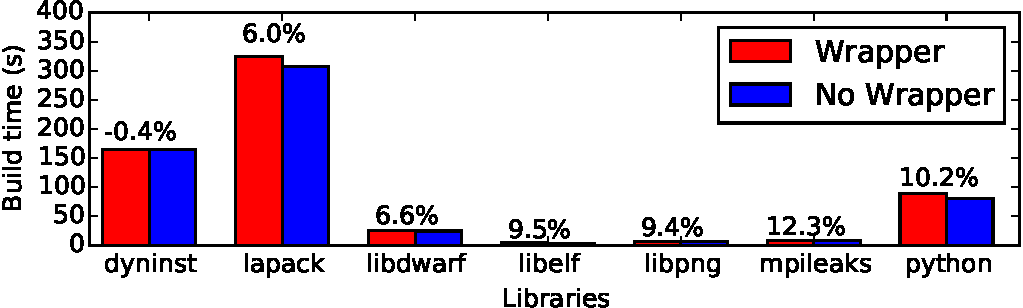
\includegraphics[width=\columnwidth]{figs/wrappers/wrapper-overhead.pdf}
	\caption{
		Build times with and without compiler wrappers\newline
		(\% overhead above bars).
		\label{fig:wrapper-overhead}
	}
\end{figure}

Argument parsing and indirection cause Spack's compiler wrappers to incur a small
but noticeable performance overhead.  Figure~\ref{fig:wrapper-overhead} shows build times
with and without the wrappers for seven different packages. Above each set of bars,
the percent overhead is written. The {\tt dyninst} and {\tt lapack} packages
use CMake to build, while the rest of the packages use autotools.
The relative overheads range from negligible (-0.4\%) in the case of {\tt dyninst},
and they are more exaggerated for shorter builds like {\tt mpileaks}, which
incurs 12.3\%.

\subsubsection{Environment Module Integration}
\label{sec:envmodule}
In addition to managing the build-time environment, Spack can assist in managing
the run-time environment.  A package may need environment variables like {\tt PATH},
{\tt MANPATH}, or {\tt PKG\_CONFIG\_PATH} set before it can be used.
As discussed in Section~\ref{sec:motivation}, many sites rely on environment
modules to setup the runtime environment.  Spack can automatically create simple
dotkit~\cite{dotkit} and Module configuration files for its packages, allowing
users to setup their runtime environment using familiar systems.  While Spack
packages do not {\tt LD\_LIBRARY\_PATH} to run, we set it in our generated module
files as well, because it can be used by build systems to find libraries, as well
as by dependent packages that do not use {\tt RPATH}.
%
Future versions of Spack may also allow the creation of Lmod~\cite{mclay:lmod}
hierarchies, as discussed in Section~\ref{sec:env-rpath}. Spack's rich
dependency information would allow such hierarchies to be generated automatically.












